%% $RCSfile: proj_report_outline.tex,v $
%% $Revision: 1.3 $
%% $Date: 2016/06/10 03:41:54 $
%% $Author: kevin $

\documentclass[11pt
              , a4paper
              , oneside
              ]{report}


\usepackage{float} % lets you have non-floating floats
\usepackage{url} % for typesetting urls
\usepackage{graphicx}
\usepackage{subcaption}
\usepackage[table,xcdraw]{xcolor}
\usepackage{hyperref}
\usepackage{titlesec}

\setlength{\parindent}{0pt}

\usepackage{titlesec}
\titleformat{\chapter}[hang] 
{\normalfont\huge\bfseries}{\chaptertitlename\ \thechapter:}{1em}{} 

%
%  We don't want figures to float so we define
%
\newfloat{fig}{thp}{lof}[chapter]
\floatname{fig}{Figure}

%% These are standard LaTeX definitions for the document
%%                            
\title{Instrumentation System for Liquid Drop Impact and Evaporation}
\author{Daniel Eisen}

%% This file can be used for creating a wide range of reports
%%  across various Schools
%%
%% Set up some things, mostly for the front page, for your specific document
%
% Current options are:
% [ecs|msor|sms]          Which school you are in.
%                         (msor option retained for reproducing old data)
% [bschonscomp|mcompsci]  Which degree you are doing
%                          You can also specify any other degree by name
%                          (see below)
% [font|image]            Use a font or an image for the VUW logo
%                          The font option will only work on ECS systems
%
\usepackage[image,ecs]{vuwproject}

% You should specifiy your supervisor here with
\supervisor{Dr. Gideon Gouws}
% use \supervisors if there is more than one supervisor

\otherdegree{Bachelor of Engineering with Honours}

% Unless you've used the bschonscomp or mcompsci
%  options above use
%   \otherdegree{OTHER DEGREE OR DIPLOMA NAME}
% here to specify degree

% Comment this out if you want the date printed.
\date{}


\begin{document}

% Make the page numbering roman, until after the contents, etc.
%\frontmatter

%%%%%%%%%%%%%%%%%%%%%%%%%%%%%%%%%%%%%%%%%%%%%%%%%%%%%%%

%%%%%%%%%%%%%%%%%%%%%%%%%%%%%%%%%%%%%%%%%%%%%%%%%%%%%%%

\begin{abstract}
    //TODO rewriting
    
    \textit{Droplet impact and evaporation presents a complex physical process worth investigating not only from a fundamental research perspective but also in its potential for industrial application. However, in order to extract usable data from this small scale, fast phenomenon in the lab producing a droplet of repeatable volume and position as well as accucartly track and collect the data (temperature, impact, evaporation) is essential in order to extract reliable and study worthy results. This procedure form the basis of this project.
    This projects approach is to add motorised automation to droplet dispensing with aims to control for droplet volume, positional variation, contact angle and speed up the procedure and allow for greater flexibility in the experimental process.}


\end{abstract}

%%%%%%%%%%%%%%%%%%%%%%%%%%%%%%%%%%%%%%%%%%%%%%%%%%%%%%%

\maketitle

\tableofcontents

%%%%%%%%%%%%%%%%%%%%%%%%%%%%%%%%%%%%%%%%%%%%%%%%%%%%%%%

\mainmatter

%%%%%%%%%%%%%%%%%%%%%%%%%%%%%%%%%%%%%%%%%%%%%%%%%%%%%%%

% individual chapters included here
\chapter{Introduction}\label{C:intro}
The investigation of droplet impact and evaporation is an area of experimentation of interest and application to various industry. Such as milk powder spray drying, ink jet printing, and applications of evaporative cooling. This project will continue on from a previous instrumentation setup, evaluate its shortcomings, and design the next generation to improve the reliability and usability of the collected data and introduce methods of automating the process. 

Report covers the key problem the experimental setup that the project aims to improve, and what are the main factors that can introduce variation into the results. An overview and evaluation of the current/previous system and the variability of its results and possible sources of that inconsistency. It was briefly cover other similar systems in literature can what they control/how. Then it will redefine the project scope, its objectives and what variables its aim to control and how. Finally it will cover what work has been down and where the current progress and results stand as well as detailing difficulties/decisions made along then way.  

\section*{The Experiment}

A droplet of liquid (concentrated milk, water, etc) is deposited on a heated substrate (stainless steel, copper, glass). The temperature of the substrate in monitored, along with the progression of the droplets impact and evaporation being captured with 2 cameras; above and profile. This produces a multidimensional perception of the developing behaviour and characteristics of the droplet over time. This usually take 1-2mins per droplet.

\subsection*{Problems}

Such a process
\chapter{Background}\label{C:back}

\section{Instrumentation and Current System}

\section{Other Approaches}
In literature, there exists a variety of rigs for similar experiments. These were explored to gauge a range of what factors were controlled (and measured) and with what approaches. In summary:
\begin{itemize}
    \item Controlled environmental factors with basic box \cite{step_book} or measured factors only \cite{measure_only}.
    \item Controlled for droplet position and volume with hard mounted pump plus needle, but lacks environmental control or automation, and there is no top view camera \cite{non_newt} \cite{fixed_pump}.
    \item Incorporated stepper motor driven automation, but no environmental control or monitoring \cite{motors}.
    \item Full environmental chamber and fixed droplet pump, but single camera, has separate uncontrolled rig for top view \cite{duel_rig}.
\end{itemize}

\newpage
\section{Background on Stepper motor control}
This section will cover the background of controlling bipolar stepper motors via a step/direction style driver setup, as its concepts will be mentioned later in the report. This is a focused background on the key considerations and requirements when designing for and operating this specific subset, and by no means applicable to all driving and specific motor choices.

The stepper motors provide precise positioning and are capable of moving their rotor to a specified position and holding that position at a wide range of load torques. This capability makes the stepper motors popular in optics, medical instruments, factory automation, and industrial equipment.

The typical topology of a stepper driving system (based around the step/direction method) consists of a controller, driver, and stepper motor. The controller provides a direction signal and step pulses, while the driver converts these signals into actual electrical power and supplies them to the motor. The stepper motor moves in steps, each step covering one step angle, which can be described as the rotor displacement corresponding to one step pulse \cite{step_app}.

Stepper motors typically have a step size specification (e.g. 1.8° or 200 steps per revolution), which applies to full steps. Step/direction drivers usually provide a 'microstepping' mode which increases the resolution by allowing intermediate step locations, which are achieved by energising the coils with intermediate current levels \cite{step_book}.

The last major consideration in driving steppers is controlling the start-up and stopping speeds for the controller's provided pulse train to the driver. As the motor is a mechanical device in the real world, expecting a perfect impulse response will lead to driving failure. Inertia ratio is critical to stepper motor acceleration \cite{step_book}. Too great a difference in inertia ratio between system and motor risks missed steps or stalling the coils. So when starting a stepper motor, acceleration and deceleration should happen through pulses to the motor that start slowly and gradually quicken in a process called ramping.


\chapter{Inital Evaluation}\label{C:init_eval}


\section{Current Experimental Setup}
The instrumentation as exists is assembled with an optical breadboard and XYZ+R stages with micrometre controls. A central stage holds the substrate with internally mounted thermocouple. Two manual focus cameras are positioned in profile and top down views, and the droplet is dispensed manually via a syringe mounted horizontally to a XYZ+R stage.
The current procedure is a manual process. The syringe tip is rotated above a marked point on the substrate, and hand emptied and refilled. This results in volume and positional variation between runs. This procedural variance is the focus of this project.

\section{Repeatability and Reliability}

Data taken from a series of five droplet runs was analysed to extract the variety in droplets and its effect on the measure temperature profile. 

\begin{figure}[h]
    \begin{center}
        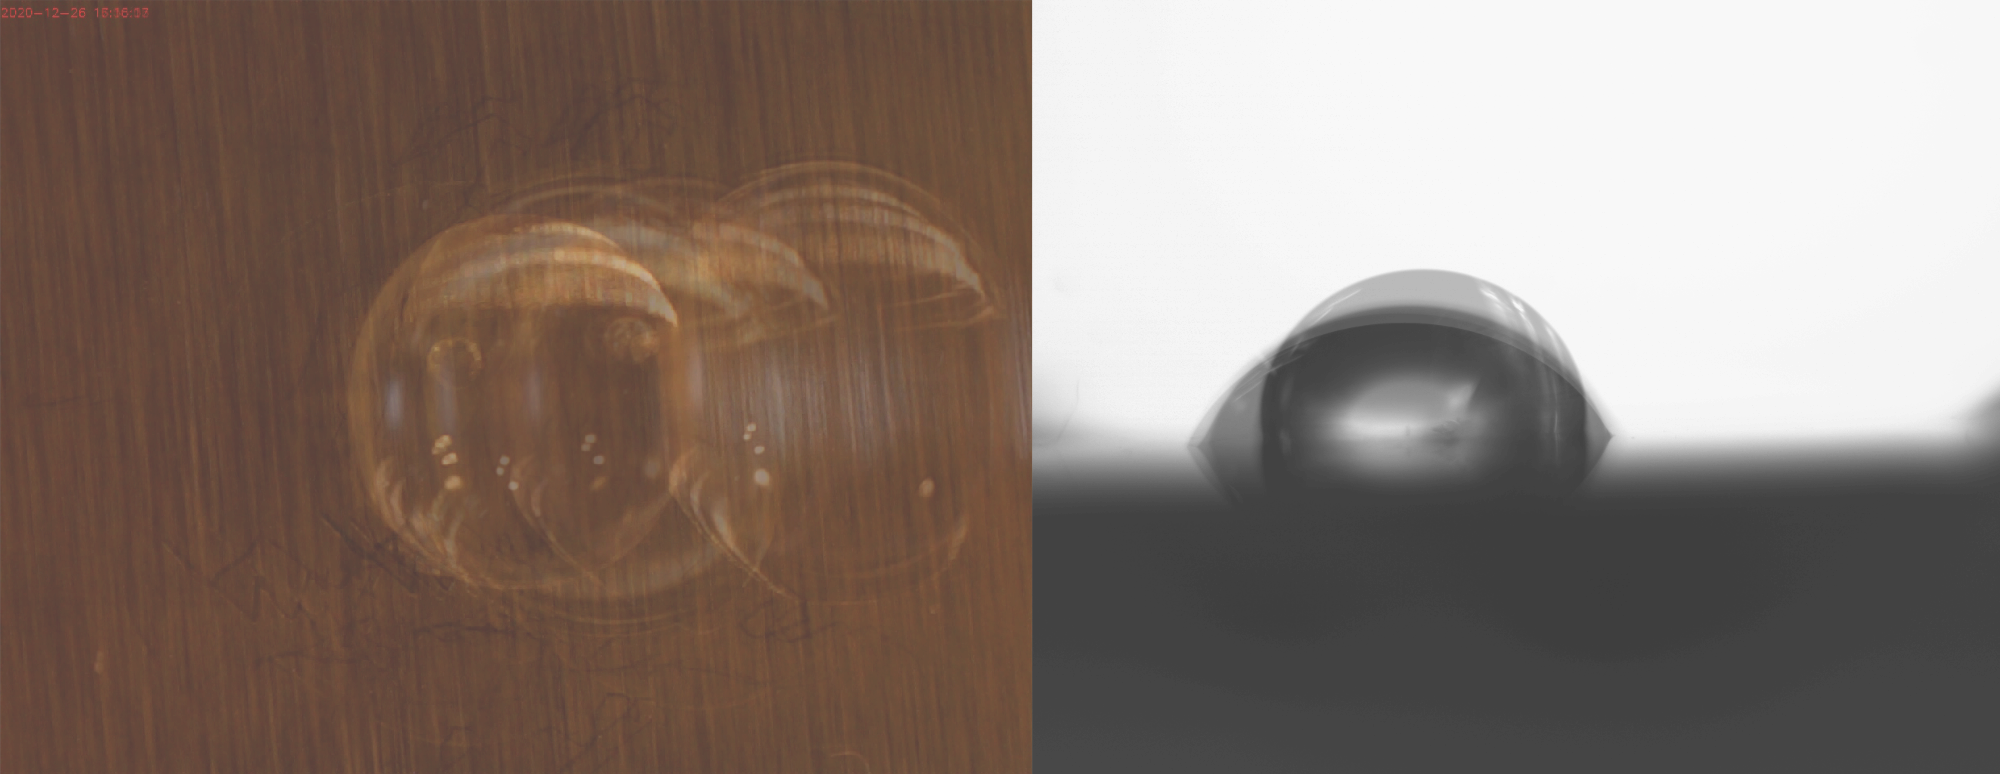
\includegraphics[width=.4\textwidth]{img/droplets_2018.png}
        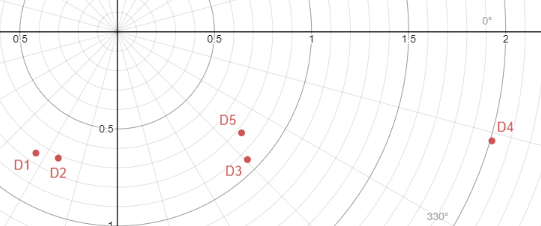
\includegraphics[width=.4\textwidth]{img/drop_pos_2018.png}

        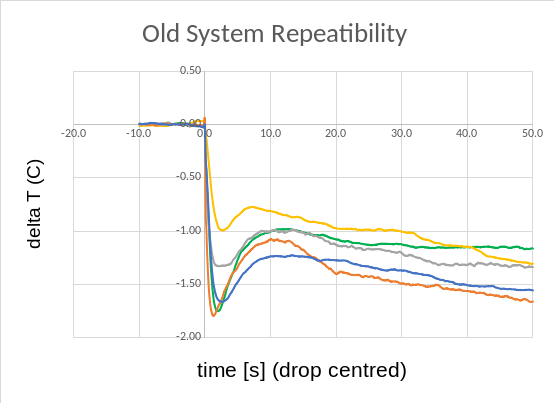
\includegraphics[width=.4\textwidth]{img/drop_temps_2018.png}
        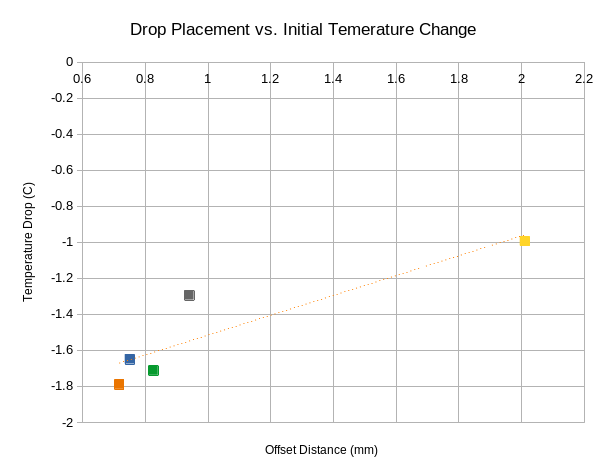
\includegraphics[width=.4\textwidth]{img/2018_pos_temp_trend.png}
    \end{center}
\end{figure}

\begin{table}[h]
    \centering
    \begin{tabular}{|l|l|l|}
    \hline
    \textit{\textbf{Droplet}} & \textit{Distance from Centre (mm)} & \textit{Estimated Volume (mm\textasciicircum{}2)} \\ \hline
    \cellcolor[HTML]{9698ED}1 & 0.7506                             & 16.55                                             \\ \hline
    \cellcolor[HTML]{E9AD3F}2 & 0.7164                             & 17.91                                             \\ \hline
    \cellcolor[HTML]{C0C0C0}3 & 0.9402                             & 17.89                                             \\ \hline
    \cellcolor[HTML]{FFFC9E}4 & 2.0104                             & 17.57                                             \\ \hline
    \cellcolor[HTML]{79CD5D}5 & 0.8258                             & 16.21                                             \\ \hline
    \end{tabular}
    \end{table}

\begin{table}[h]
    \centering
    \begin{tabular}{|l|l|l|}
    \hline
                   & \textit{Distance from Mark}          & \textit{Measured Temperature Drop} \\ \hline
    Min Pos Offset & 0.71mm                     &-1.7901$^{\circ}C$    \\ \hline
    Max Pos Offset &       2.01mm    &  -0.9944$^{\circ}C$    \\ \hline
                   & \textit{Volume}            & \textit{Contact Angle}          \\ \hline
    Shape Variance & $0.629mm^3$ & 25.894 degrees $\dagger$                \\ \hline
    \end{tabular}
    \caption{Variance in Setup}
    \subcaption*{$\dagger$This excluded an outlier of an almost spherical droplet with contact angles exceeding 95 degrees. This large variation is most likely due to inconsistency in surface chemisty from washing.}
    \end{table}


\section{Revised Approach}
The focus of the project is now twofold. Firstly on the automation of the process to allow for faster, pre-programmed runs to be carried out easier, and secondly to improve on the repeatability and reliability of the results by controlling the procedural factors of the experiment. 

\begin{table}[h]
    \begin{tabular}{lll}
    \textbf{Effector} & \textbf{Likelihood} & \textbf{Effect Strength} \\
    Position          &                    &                          \\
    Volume            &                    &                          \\
    Contact angle*    &                    &                          \\
    Humidity          &                    &                          \\
    Temperature       &                    &                          \\
    Pressure          &                    &                         
    \end{tabular}
    \end{table}

An electronic pipette will be used to dispense a precise volume, and motorised stages will be used to provide preprogrammed, repeatable motion. The environmental factors however are not to be ignored, though controlling them is outside of the scope of this project. They will, however, be monitored, and this project will implement data collection of temperature, atmospheric pressure and humidity so these factors can be correlated to any remaining variation in data.  w
\chapter{Design}\label{C:des}

\section{Project Specifications and Justifications}
Given the results of the initial evaluation the project can now be constrained. It's main goals are to eliminate volume variation, control for droplet position, enable automation to reduced time between consecutive runs. It will not control, but provide data-logging for the environmental effectors; temperature, humidity, pressure.

From this there is a number of requirements to consider:

\begin{itemize}
    \item \textbf{Mechanical Stability}:
    \item \textbf{Droplet Position Repeatability}
    \item \textbf{Consistent Volume}
    \item \textbf{Process Automation}
    \item \textbf{System Expandability}:
\end{itemize}

The project will be evaluated on how it meets the above Specifications, its ability to control for volume and positional accuracy and repeatability as well as how it adds/improves automation, provides environmental data and allows extension.


\section{Volume Control}

In order 


\section{Mechanical Design}

\begin{itemize}
    \item Discuss requirements for minimising settling time, vibrations, oscillations.overshoot of the pipette motion
\end{itemize}


\subsection{Rotating Pipette Mount}

\begin{itemize}
    \item 3D printed pipette clamp
    \item Laser cut Tower mounted
    \item motor interface and stage fastening
\end{itemize}

The electronic pipette formfactor is very 'organic', so the clamping mechanism to fit it to the tower plate itself was challenging to design to successfully restrict its rotation and backlash.
The base design used to accomplish this was a 3D-printed ring clamp meant to be tightened and fit to the unique form of the pipette body. A variety of ring sizes and gap distance were printed and test fitted. From this it was determined that a ring diameter of 32mm and a gap of 6mm fits and deforms to the shape of the pipette. However, there was still some rotation and slip so a notch was cut into the acrylic to slot the pipettes support rest and a second ring clamp (36mm) attached lower down of the body.

\subsection{Z micrometer Control}

In order to control the the height of the pipette tip; to enable automated refilling and to place the dispensed droplet on to the substrate the Z height of the optical stage needs to be motorised. The Z height has a manual control in the form of an adjustment micrometer that allows for 10mm of travel, but this present the first problem in design.
The micrometer travels linearly throughout the adjustment, i.e. if the stage raises 10mm the knob will retract 10mm also. Due to this a custom shaft coupler is required to interface a fixed motor to the moving knob.

\begin{figure}[h]
    \centering
    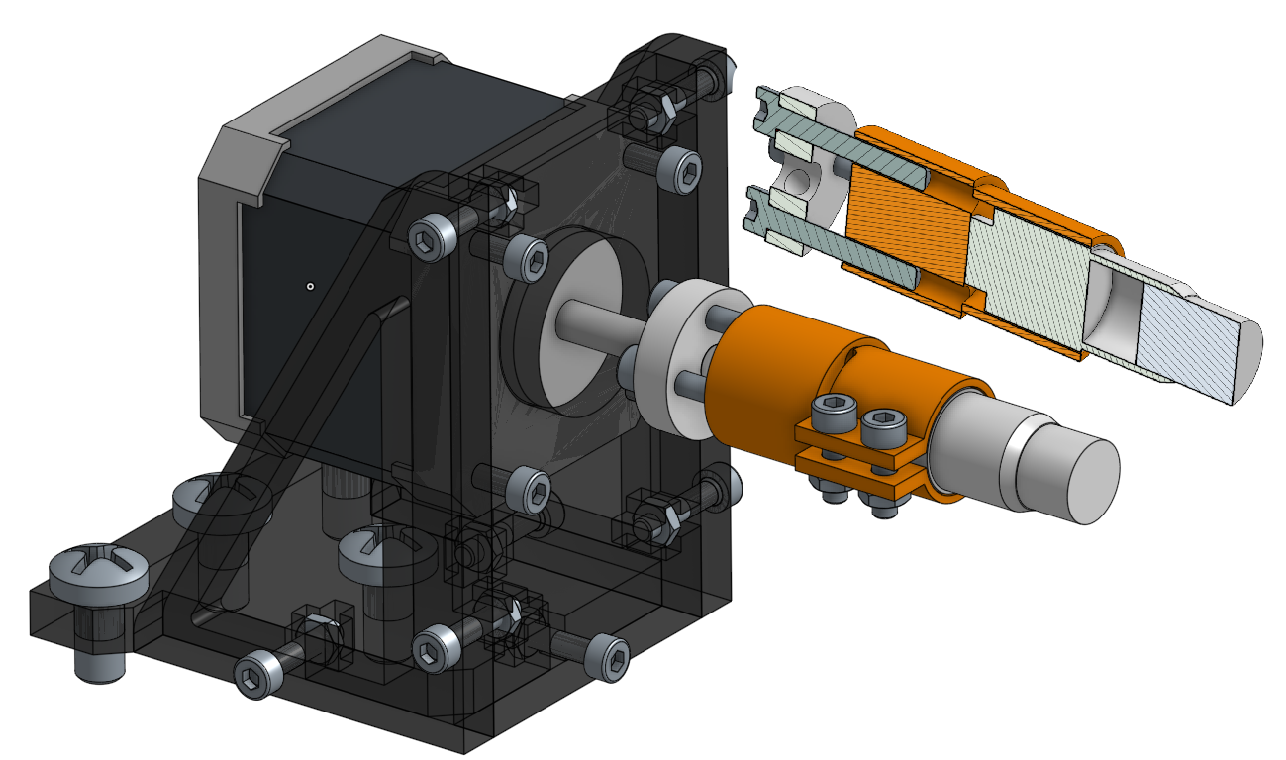
\includegraphics[width=0.4\textwidth]{img/z_control.png}
    \caption{Z driving motor and sliding shaft coupler}
    \label{fig:z_coup}
\end{figure}

The figure above[\ref{fig:z_coup}] shows the assembled design. One end of the coupler is an extended c-clamp that mates with the knurls knobs of the micrometer and the other is a solid piece with 4 M3 clearance holes. These holes interface with a universal shaft-hub mount with 4 M3 machine screws that transfer the motors rotation and allow the coupler and knob to slide away over the course of a movement.

The key limitation of this design is that is constrains the XY position of the stage to a single setting. This is due to the motor being fastened to the breadboard baseplate more stability, alignment and vibration reduction. Because of this it moves the fine positioning to the other stages in the setup; substrate stack and cameras. 

\section{Electronic Design}

\subsection{Motors}
The motion required for the motors in this system is to provide rotation about the vertical axis to the mounted pipette, to swing from above the substrate to out of the camera view and over a refill reservoir, as well as continuous rotation to interface the Z axis control for droplet depositing and possible refilling.

Stepper motors allow for both precise position control without the need for a feedback system and are capable of continuous rotation. In comparison, brushed/brushless DC motors require encoders for positional control and servos may do either but not both continuous rotation and positioning.

NEMA17 standard sized steppers were chosen to best fit the dimensions of the XYZ optical stage (60mm plate to 40mm motor frame) with room for fastening hardware. That left two choices for the top R stage motor; full size 38mm high frame or shorter pancake frame. Even through the pancake frame would reduce the overall height of the system, the shaft length available for this motor is less only 7mm and would greatly restrict the mounting options of the tower to the motor. For this reason 2 NEMA17x38mm Stepper motors were chosen.

\subsection{Motor Driving}

\subsubsection*{The Requirements}
To drive the selected stepper motors, discrete step/direction style micro stepping drivers were chosen. This allows for the design to be flexible with its electronics placed to accommodate the experimental needs. Allows for a fairly agnostic choice for controller to supply the control signals, and standardised pinouts allow for requirement flexibility and replacements.

\begin{table}[h]
    \centering
    \begin{tabular}{|l|l|l|l|l|}
        \hline
        \textbf{}     & \textbf{A4988} & \textbf{DRV8825} & \textbf{STPIN820} & \textbf{DRV8834} \\ \hline
        Step Res      & 1/16           & 1/32             & 1/256             & 1/32             \\ \hline
        Logic Level   & 3V3/5V         & 3V3/5V           & 3V3/5V            & 3V3/5V           \\ \hline
        Current Limit & 1A             & 1.5A             & 0.9A              & 1.5A             \\ \hline
        Drive Voltage & 8-35V          & 8.2-45V          & 7-48V             & 2.5-10.8         \\ \hline
    \end{tabular}
    \caption{Comparison of considered drivers}
\end{table}

Main consideration for device choice are: micro step resolution, driving current limit (passively cooled), and configuration pinout.

\subsubsection*{The Choice}
The DRV8825 was ultimately chosen.
\begin{itemize}
    \item High microstepping resolution, lower than the STPIN820 but cheap high resolution driver are prone to step skipping \cite{step_book}
    \item Highest driving current as torque requirements are unknown for this design the headroom is nice even if it isn't use, especially as it will run cooler at lower power draw.
    \item It ranked above the DRV8834 due to it configuration pins (to set microstepping mode) as it provide all 3 pins without the requirement to leave pins floating as a setting thus allowing for full software control.
\end{itemize}

\subsection{Environmental Monitoring}

Although the aim of thid


\section{System Overview}

\begin{figure}[h]
    \centering
    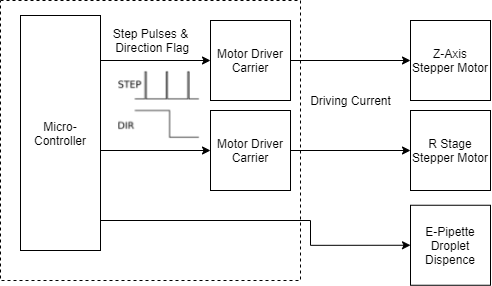
\includegraphics[width=0.4\textwidth]{img/ED_block_diag.png}
    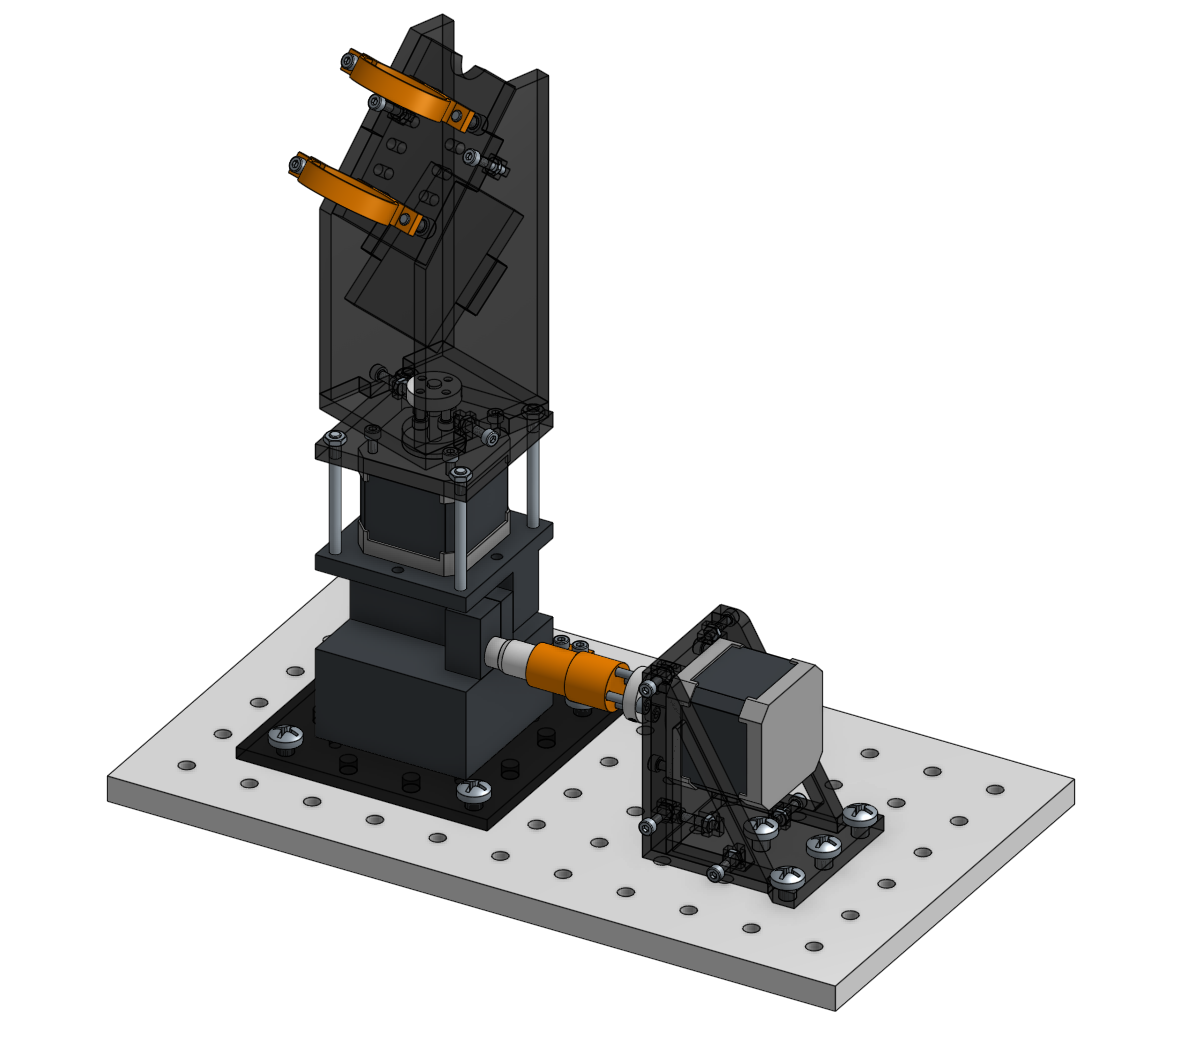
\includegraphics[width=0.4\textwidth]{img/full_mech.png}
\end{figure}
\chapter{Implementation}\label{C:imp}


//TODO rename sections to reflect work done
\section{Mechanical Design}

\begin{itemize}
    \item Go into 3d printing/laser cutting refinement, testing and adjustment
    \item Tolerance and dimension adjustment
    \item Noted changed and drawback from design
\end{itemize}

\subsection{Rotating Pipette Mount}

\subsection{Z micrometer Control}
\begin{itemize}
    \item Note initially large vibrations as z decreases, caused be loose tolerance, too small coupler. Caused droplet to prematurely detach at larger values.
\end{itemize}


\begin{figure}[h]
    \centering
    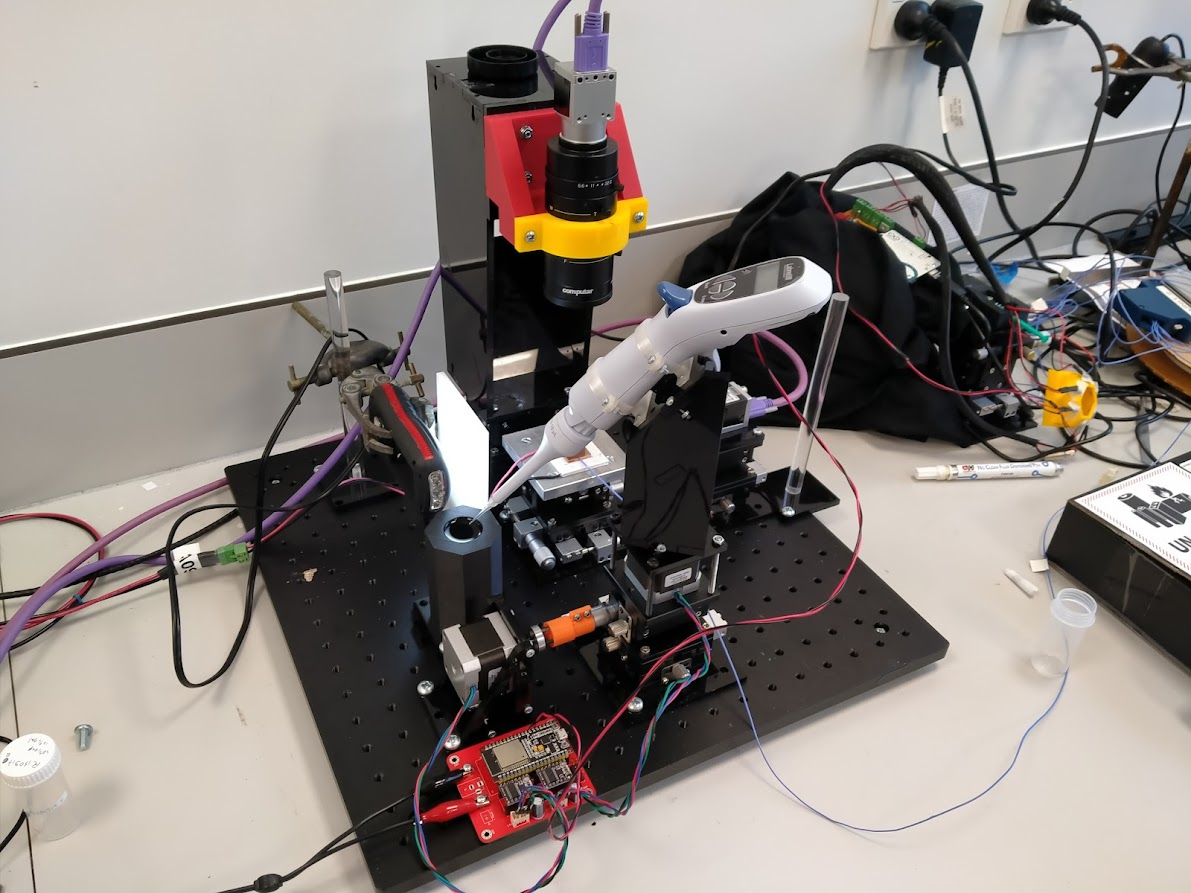
\includegraphics[width=0.4\textwidth]{img/full_sys.jpg}
    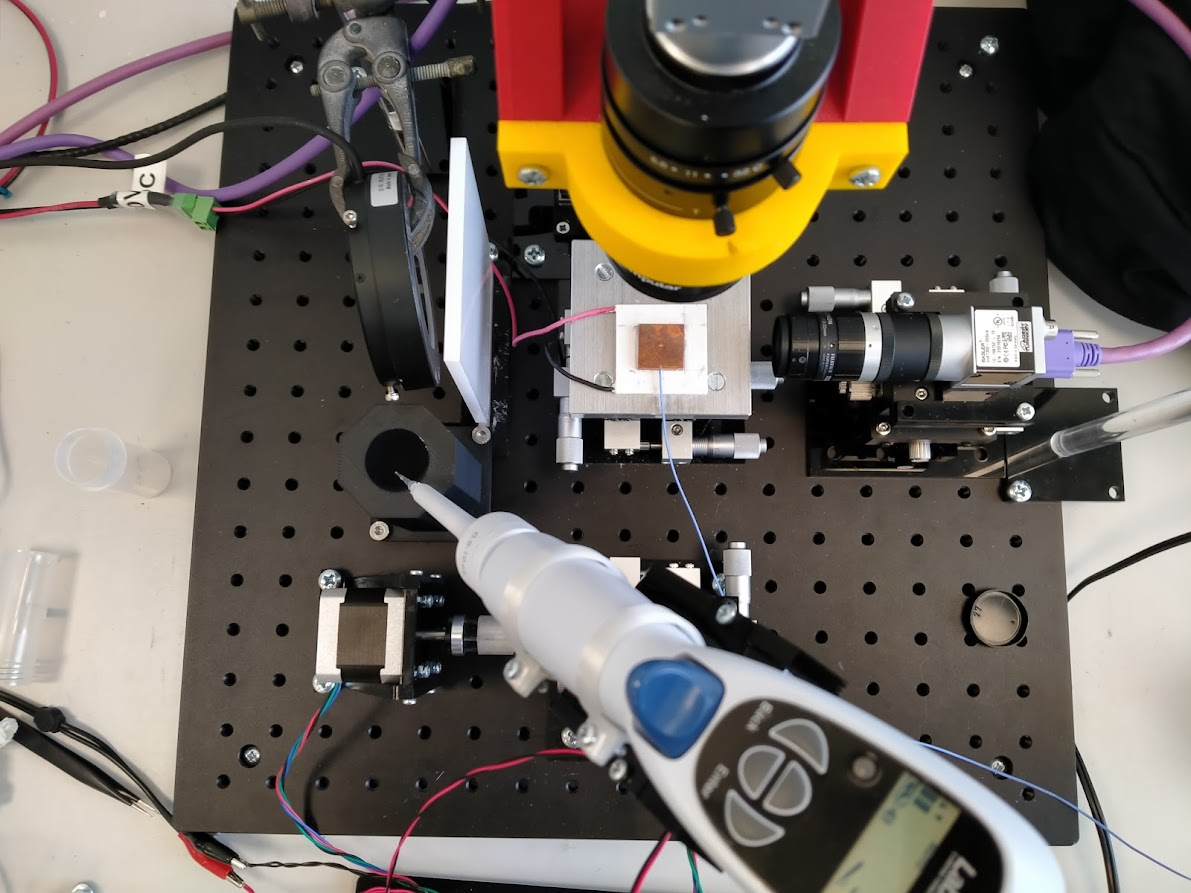
\includegraphics[width=0.4\textwidth]{img/impl_sys_top.jpg}
    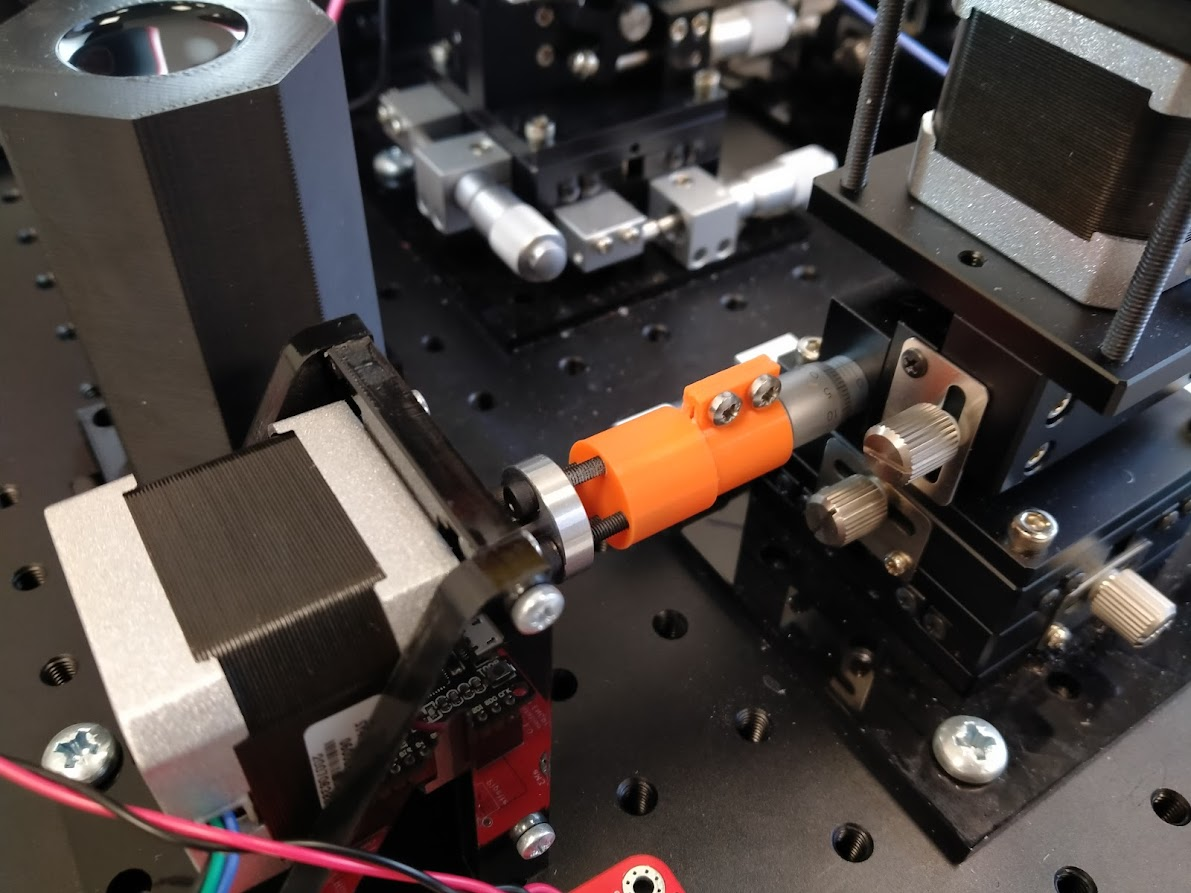
\includegraphics[width=0.4\textwidth]{img/impl_coup.jpg}
    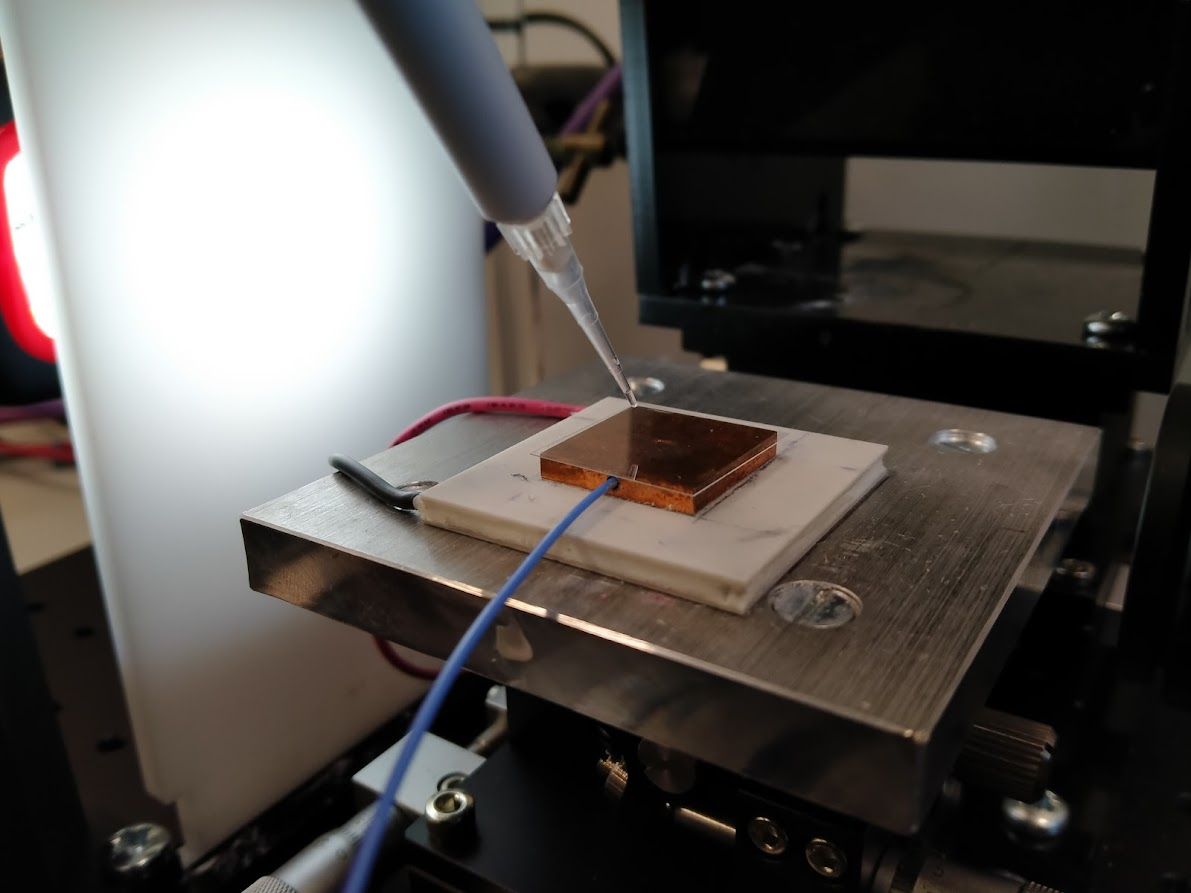
\includegraphics[width=0.4\textwidth]{img/new_stack.jpg}
\end{figure}

\section{Electronic Design}

\begin{figure}[h]
    \centering
    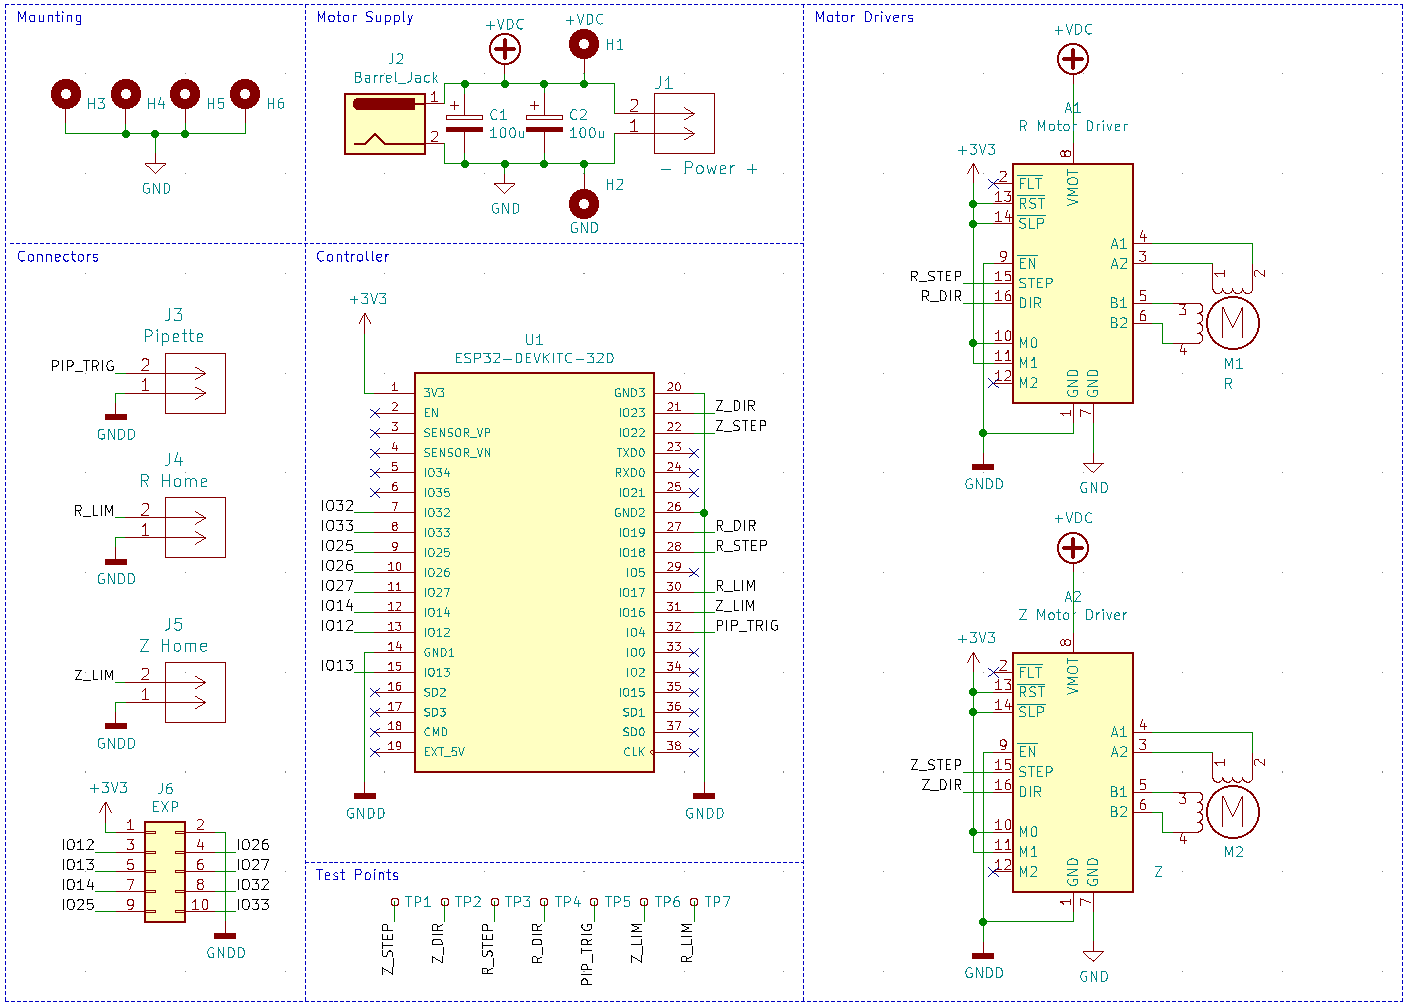
\includegraphics[width=0.4\textwidth]{img/schem.png}
    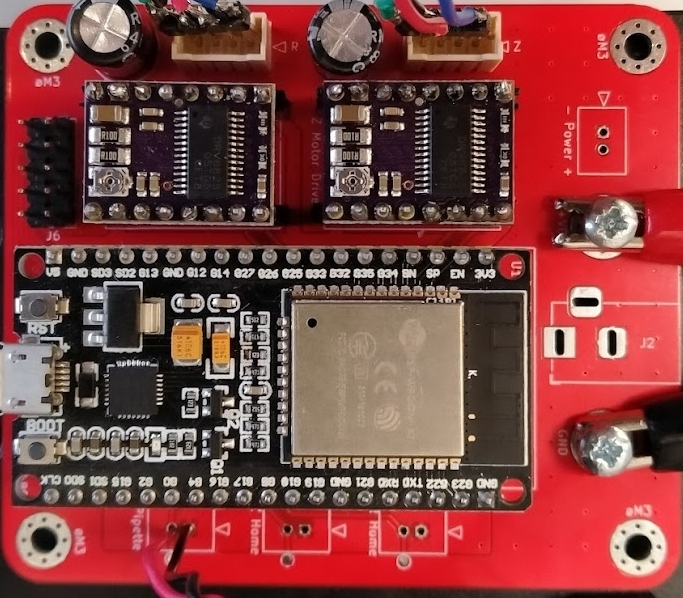
\includegraphics[width=0.4\textwidth]{img/control_pcb.jpg}
\end{figure}

\begin{itemize}
    \item full circuit
    \item pcb
    \item any and all adjustment found and made during implementation
\end{itemize}

\subsection{Motor Driving}

\subsection{Setup and Requirements}

\begin{itemize}
    \item characterised skipping issue at 100Hz, 180Hz-200hz in single step
    \item implemted micro stepping to solve
\end{itemize}

//TODO rewrite

Driving firmware was implemented on an ESP32 to validate its ability in producing the required pulse train step signal. The controller was required to produce N steps (pulses) at a set average speed, and ramp up and down that pulse speed at the head and tail of that signal.

Set values of 200 steps forward and back, at a speed of 200 steps per second, with max acceleration or 800 steps per second per second:

These pulses were captured on a second microcontroller listening for falling edges to trigger an interrupt routine to record and display that data.

\subsection{Results}

Figure \ref{fig:code}:a shows a successfully produced signal of 200 pulses with an inferred acceleration at its head/tail. This speed ramping is better illustrated in figure \ref{fig:code}:b showing the stepping change in pulses per second over the course of the pulse train.

\begin{figure}[h]
    \centering
    \begin{subfigure}{.45\textwidth}
        \centering
        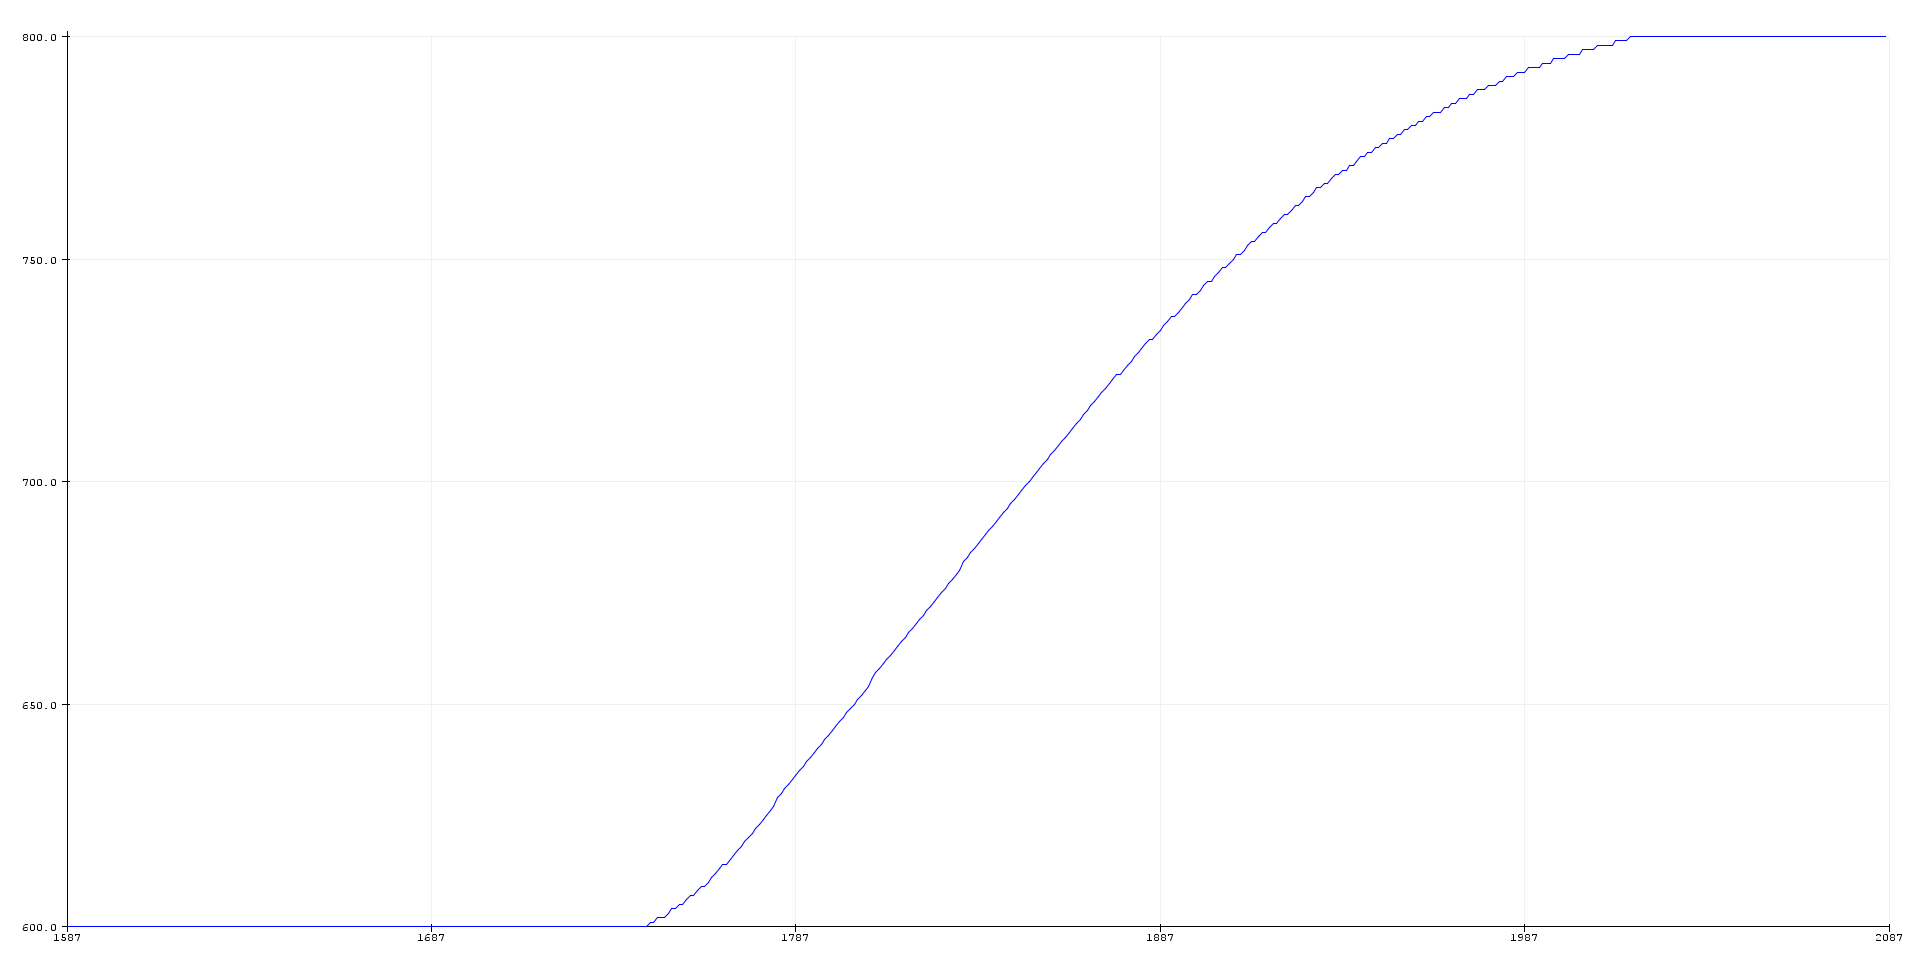
\includegraphics[width=0.8\linewidth]{img/stepper_pulses.PNG}
        \caption{Pulse Count}
    \end{subfigure}%
    \begin{subfigure}{.45\textwidth}
        \centering
        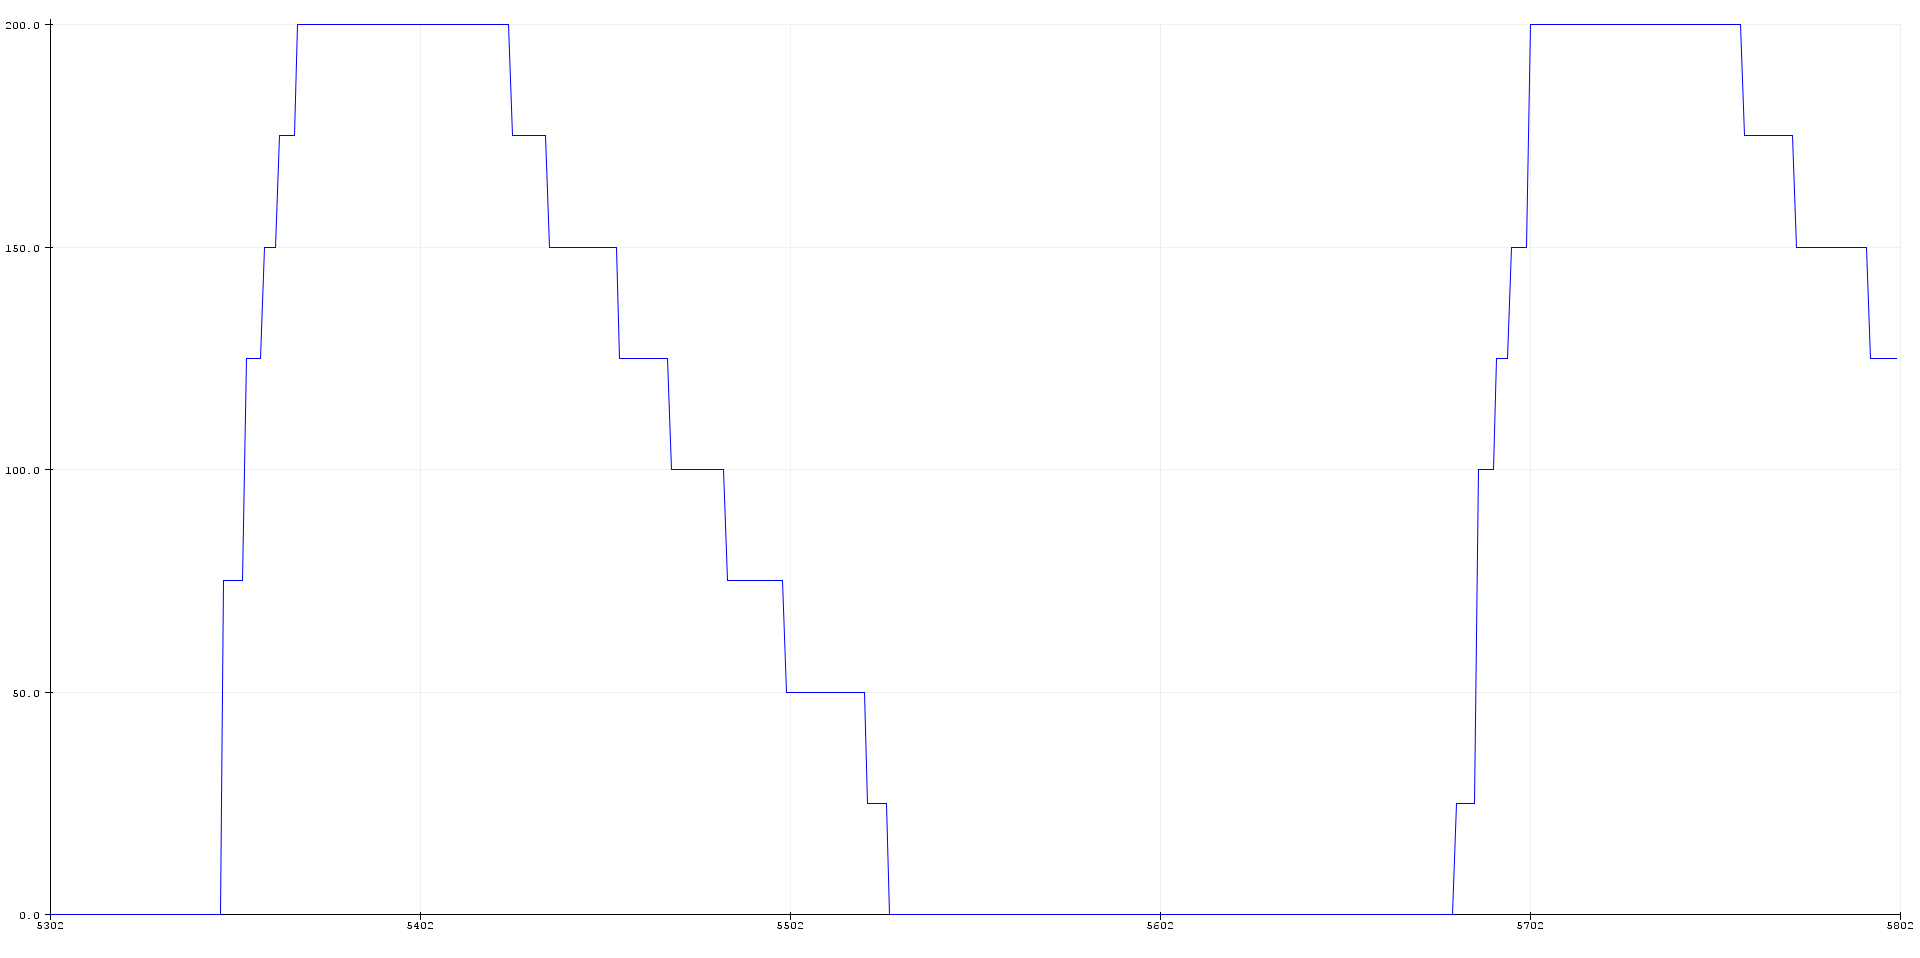
\includegraphics[width=0.8\linewidth]{img/stepper_pulse_acc.PNG}
        \caption{Pulses per Second}
    \end{subfigure}
    \caption{}
    \label{fig:code}
\end{figure}

\subsection{Pipette Triggering}

\begin{figure}[h]
    \centering
    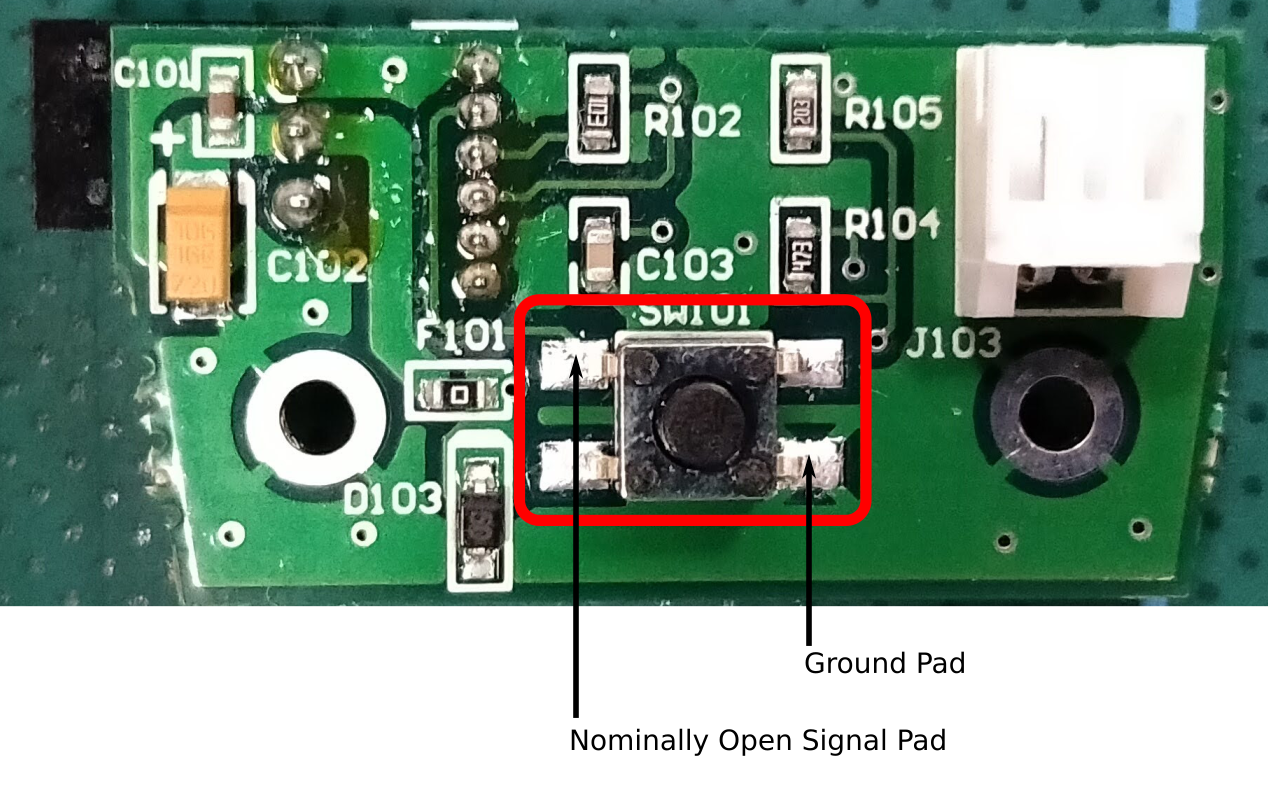
\includegraphics[width=0.4\textwidth]{img/trig_brd.png}
    \caption{E-Pipette dispensing trigger switch daughter board with exposed pads}
\end{figure}

\subsection{Environmental Monitoring}

\begin{figure}[h]
    \centering
    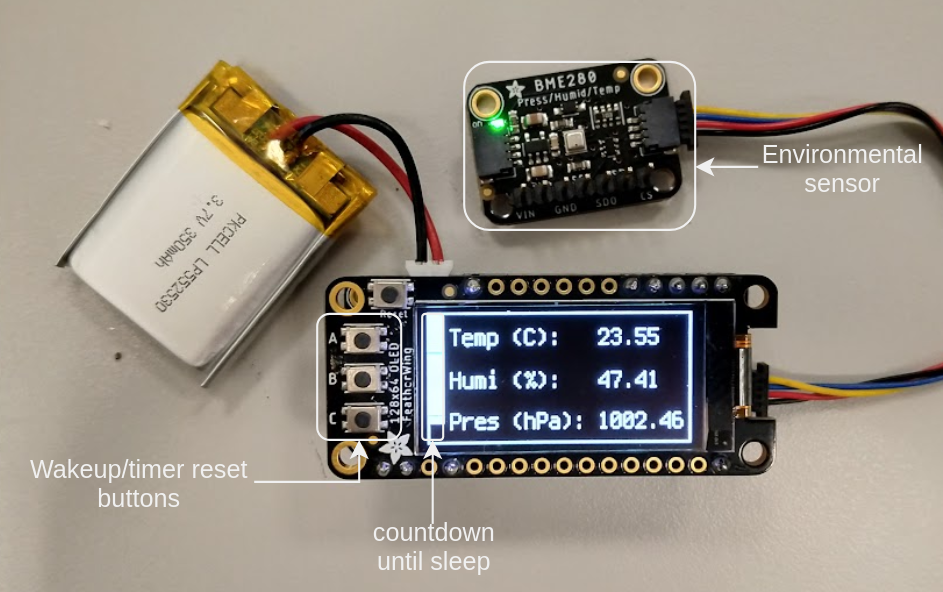
\includegraphics[width=0.4\textwidth]{img/env_mon.png}
    \caption{Implemented Environmental Monitor}
\end{figure}

\section{Software}

//Insert Serial Command Table (maybe only appendix)

\subsection{Motorised Dispensing Controller}
ESP32 based system controller with serial interface for issuing commands. Provides functionality to:
\begin{itemize}
    \item Motorised stages, height and angular position
    \item e-Pipette droplet dispensing
\end{itemize}

\subsection{Environmental Monitor}

\begin{itemize}
    \item Auto sleeping, button wake upon
    \item Circuit-Python implementation
\end{itemize}

\subsection{LabView Temperature Logger}


\chapter{Evaluation}\label{C:eval}

\section{Mechanical Stability}
Perform Motor driving parameter sweep to optimise mechanical performance according to requirements; 
of minimising pipette tip overshoot and settling time.
\subsection{Procedure}
\begin{itemize}
    \item Position tip at -1/4 revolution before zero point
    \item Set Speed/acceleration values
    \item Swing to zero position
    \item Repeat for value sleep=1rev/s, acc=1/rev/s/s $\rightarrow$  speed=2rev/s, acc=10/rev/s/s
    \item Note: acceleration is the ramp down at end/start of motion so is what we care most about
    \item Camera captured motion 
\end{itemize}



\subsection{Results}

//insert generated figures of tip position

//generated trend lines/aggregated data (settle, overshoot) from data.
\begin{figure}
    \centering
    \includegraphics[width=0.4\textwidth]{{example-image}}
\end{figure}

\section{Droplet Volume}
Something the previous system could not achieve was dispensing a variety of volumes.
Use e-pipettes programmable volume to investigate the limits of this project.
\begin{itemize}
    \item How large a droplet can be held on to? (prelim: 8uL)
    \item How large (over above) can reliably self release (w/out touch down)
    \item How small a droplet can be dispensed (e-pipette has draw-back).
\end{itemize}    

\begin{center}
    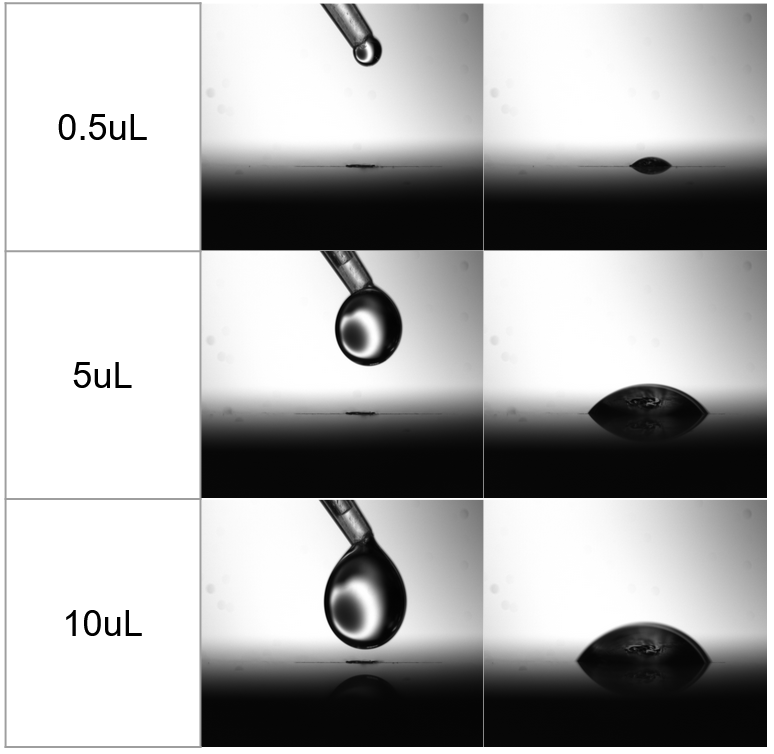
\includegraphics[width=0.4\textwidth]{img/volume_range.png}
\end{center}

\section{Repeatability and Reliability}

This section aims to produce the main set of comparable results for evaluating the projects produced system against the output of the previous setup. Thus justifying the success of one of main goals.

\subsection{Procedure}
\begin{itemize}
    \item \textbf{Initial Setup:} Roughly Position substrate stage, reservoir platform and note angular positions as well as vertical clearance requirements.
    \item \textbf{Zero System:} Using overhead camera precisely position pipette tip above substrate centre
    \item \textbf{Data Acquisition:} Initialise cameras, collect pixel:mm calibration data for analysis, initial LabView temperature logger, and environmental monitor noted. Info: temperature data rate, camera frame rate
    \item \textbf{Automated Sequence:} Via the serial link, enter the procedures command sequence to represent $\rightarrow$ lower, draw up fluid, raise, position over substrate, dispense, lower, raise, clear camera view. With appropriate delays.
    \item \textbf{Capture:} Begin data collection and automated dispense.
    \item \textbf{Repeat: } Minimum of 5 times. Each time carefully cleaning substrate surface to minimised up measured factors. 
\end{itemize}

\newpage
\subsection{Analysis and Results}

To show the system successfully increases the consistency of droplet position and investigate whether this supports the hypothesis that this resulted in better temperature consistency.

\begin{figure}[h]
    \centering
    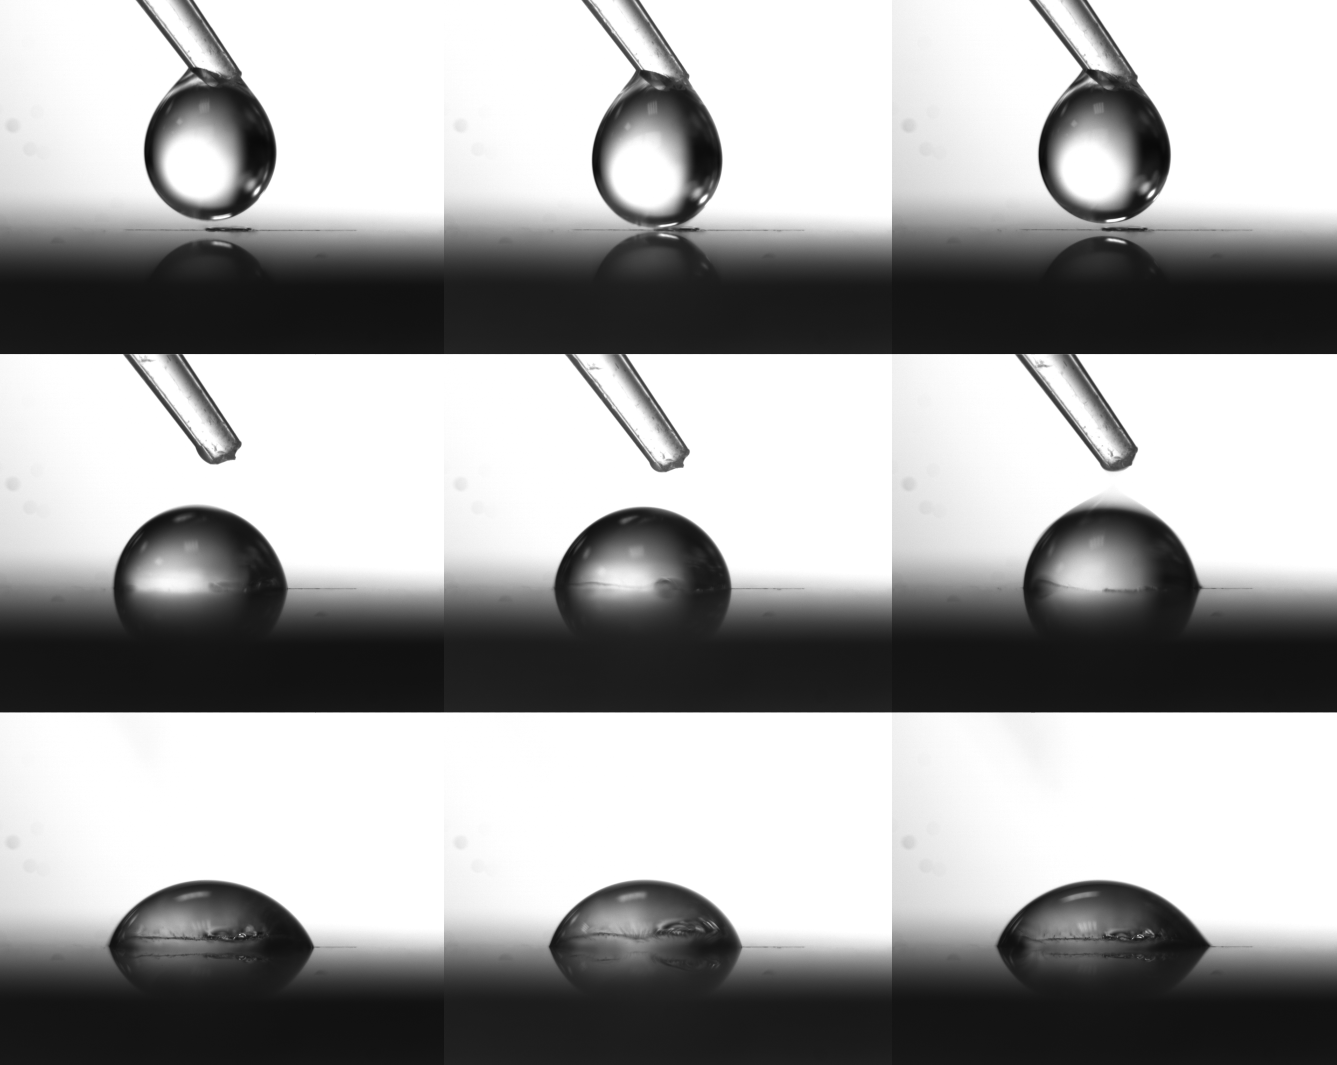
\includegraphics[width=0.4\textwidth]{img/side_drops.png}
    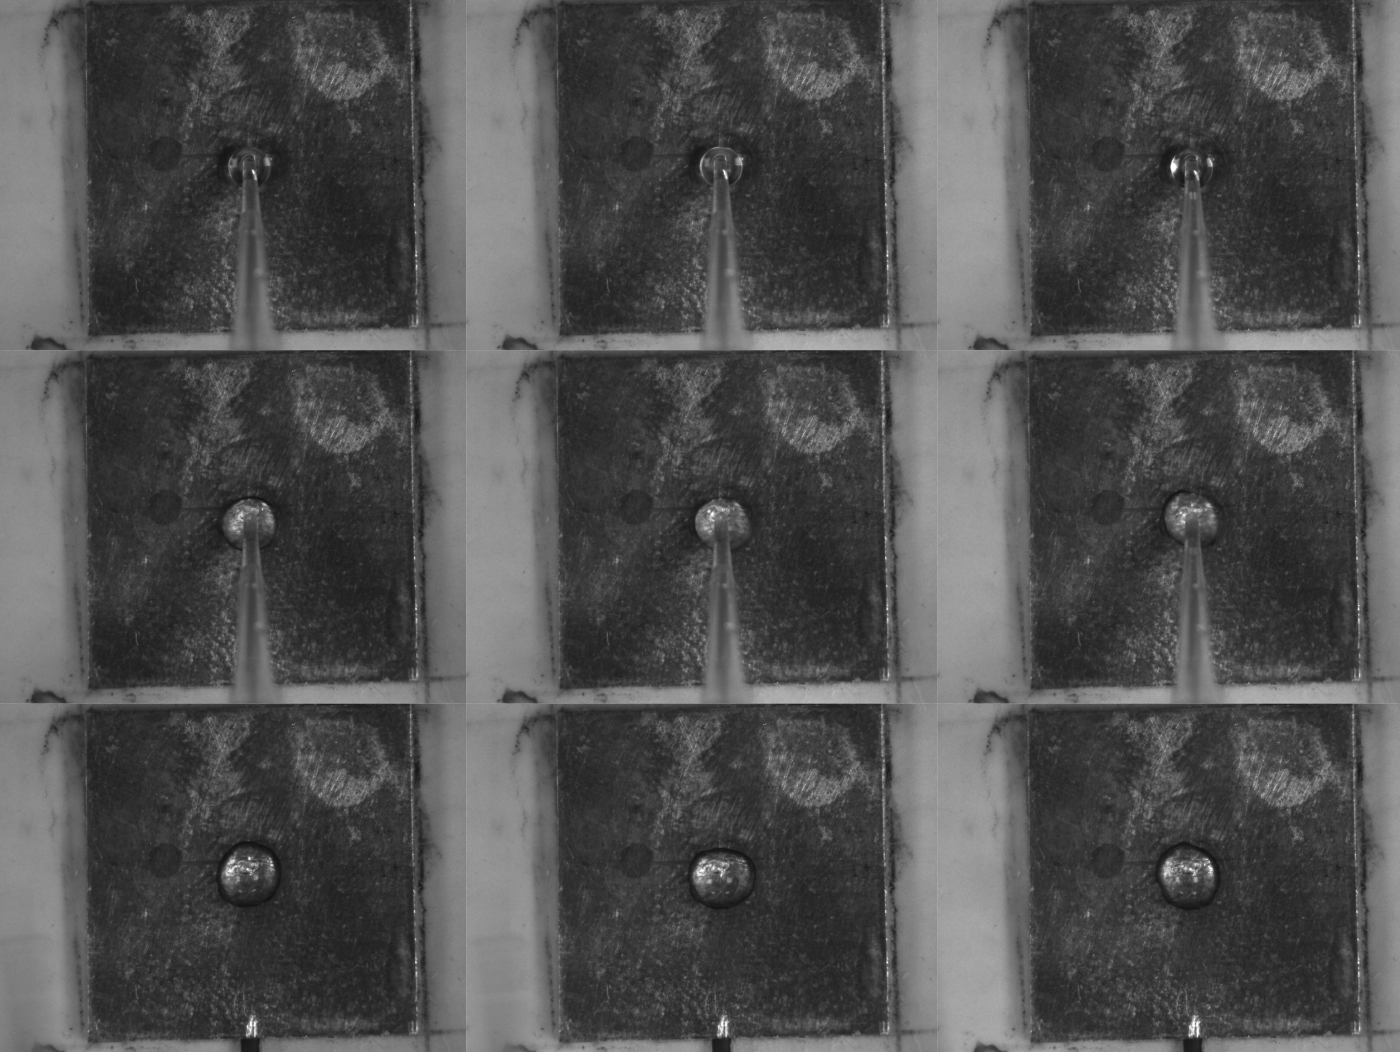
\includegraphics[width=0.4\textwidth]{img/top_drops.png}
\end{figure}

\begin{figure}[h]
    \centering
    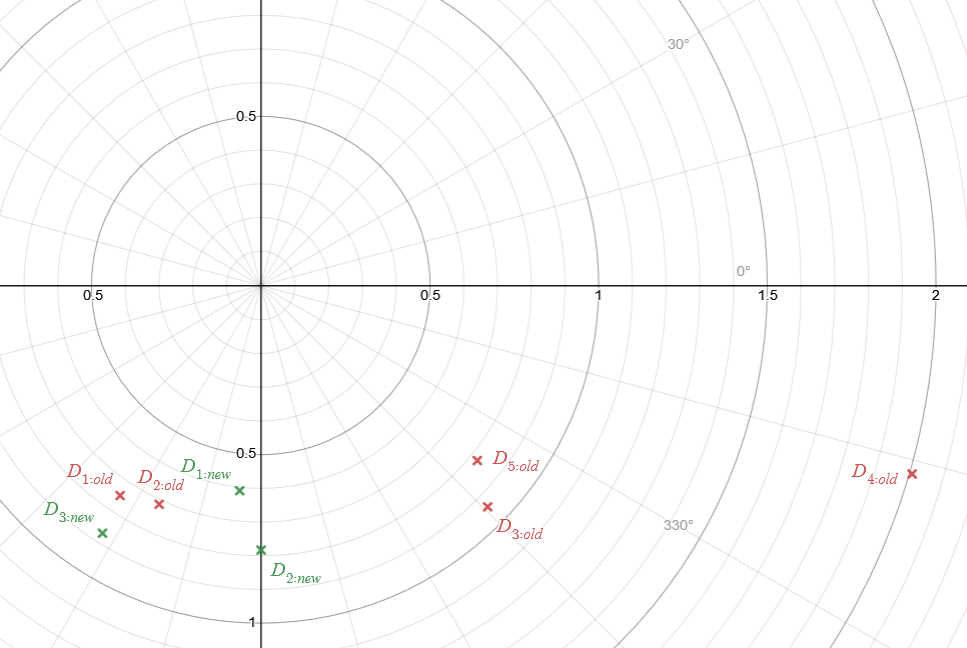
\includegraphics[width=0.4\textwidth]{img/pos_comp.png}
    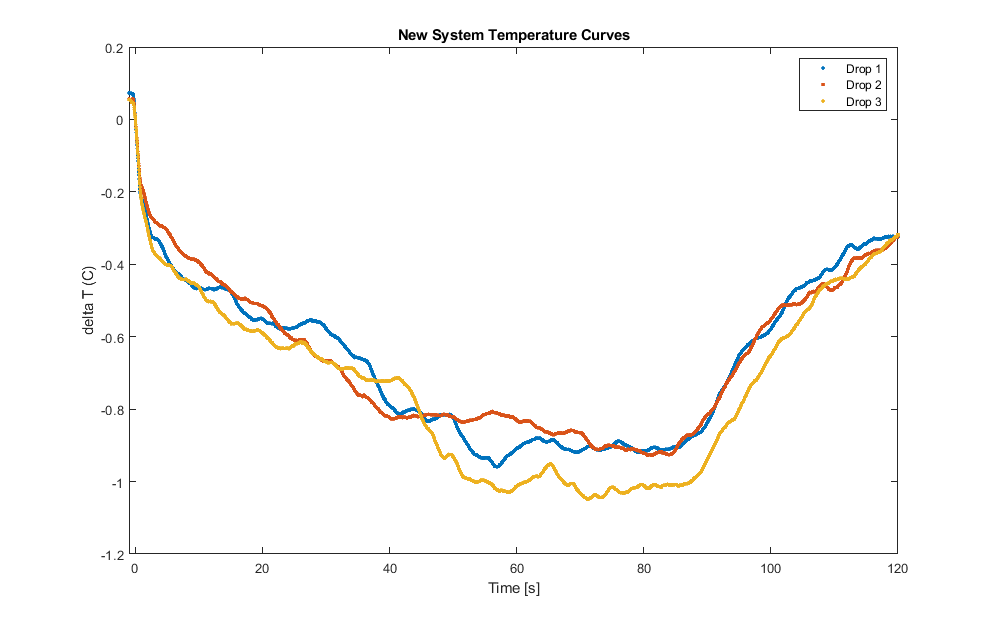
\includegraphics[width=0.4\textwidth]{img/new_temp.png}
\end{figure}


\chapter{Conclusions and Future Work}\label{C:conclusion}

Future work should not just be a list of things that you would have done if you had a little more time. Talk about new things that are possible now that you have finished your project. What projects could an ENGR489 student tackle next year if they started from your end point?

\section{Conclusion}

\section{Future Work}

%%%%%%%%%%%%%%%%%%%%%%%%%%%%%%%%%%%%%%%%%%%%%%%%%%%%%%%

\backmatter

%%%%%%%%%%%%%%%%%%%%%%%%%%%%%%%%%%%%%%%%%%%%%%%%%%%%%%%

\bibliographystyle{ieeetr}
\bibliography{bib}

\end{document}
